\subsubsection{Fra 3D-model til billede}
I dette afsnit er det vist, hvordan der kan udledes en model, der beskriver en billeddannelsen af objekter i rummet, også kaldt rendering. Dette er essentielt da billeddannelsen danner grundlag for, hvordan 3D-modellen for en lampe omdannes til et billede, der kan vises for kunderne på e-butikken. Til sidst i afsnittet udledes en model for, hvordan belysningen fra en lampe kan simuleres og visualiseres vha. raytracing. 

\paragraph{Perspektiv projektion}
For at udlede en model for billeddannelsen, tages der udgangspunkt i en perspektiv projektion. Perspektiv projektion er en måde at danne et billede af 3D-objekter ved at projektere objekterne hen på et plan mod et kameraes position\cite{fig:perspective_projection}. Princippet bag perspektiv projektion er vist på figur \ref{fig:perspektiv_projektion}.

\begin{figure}[H]
  \label{fig:perspektiv_projektion}
  \centering
  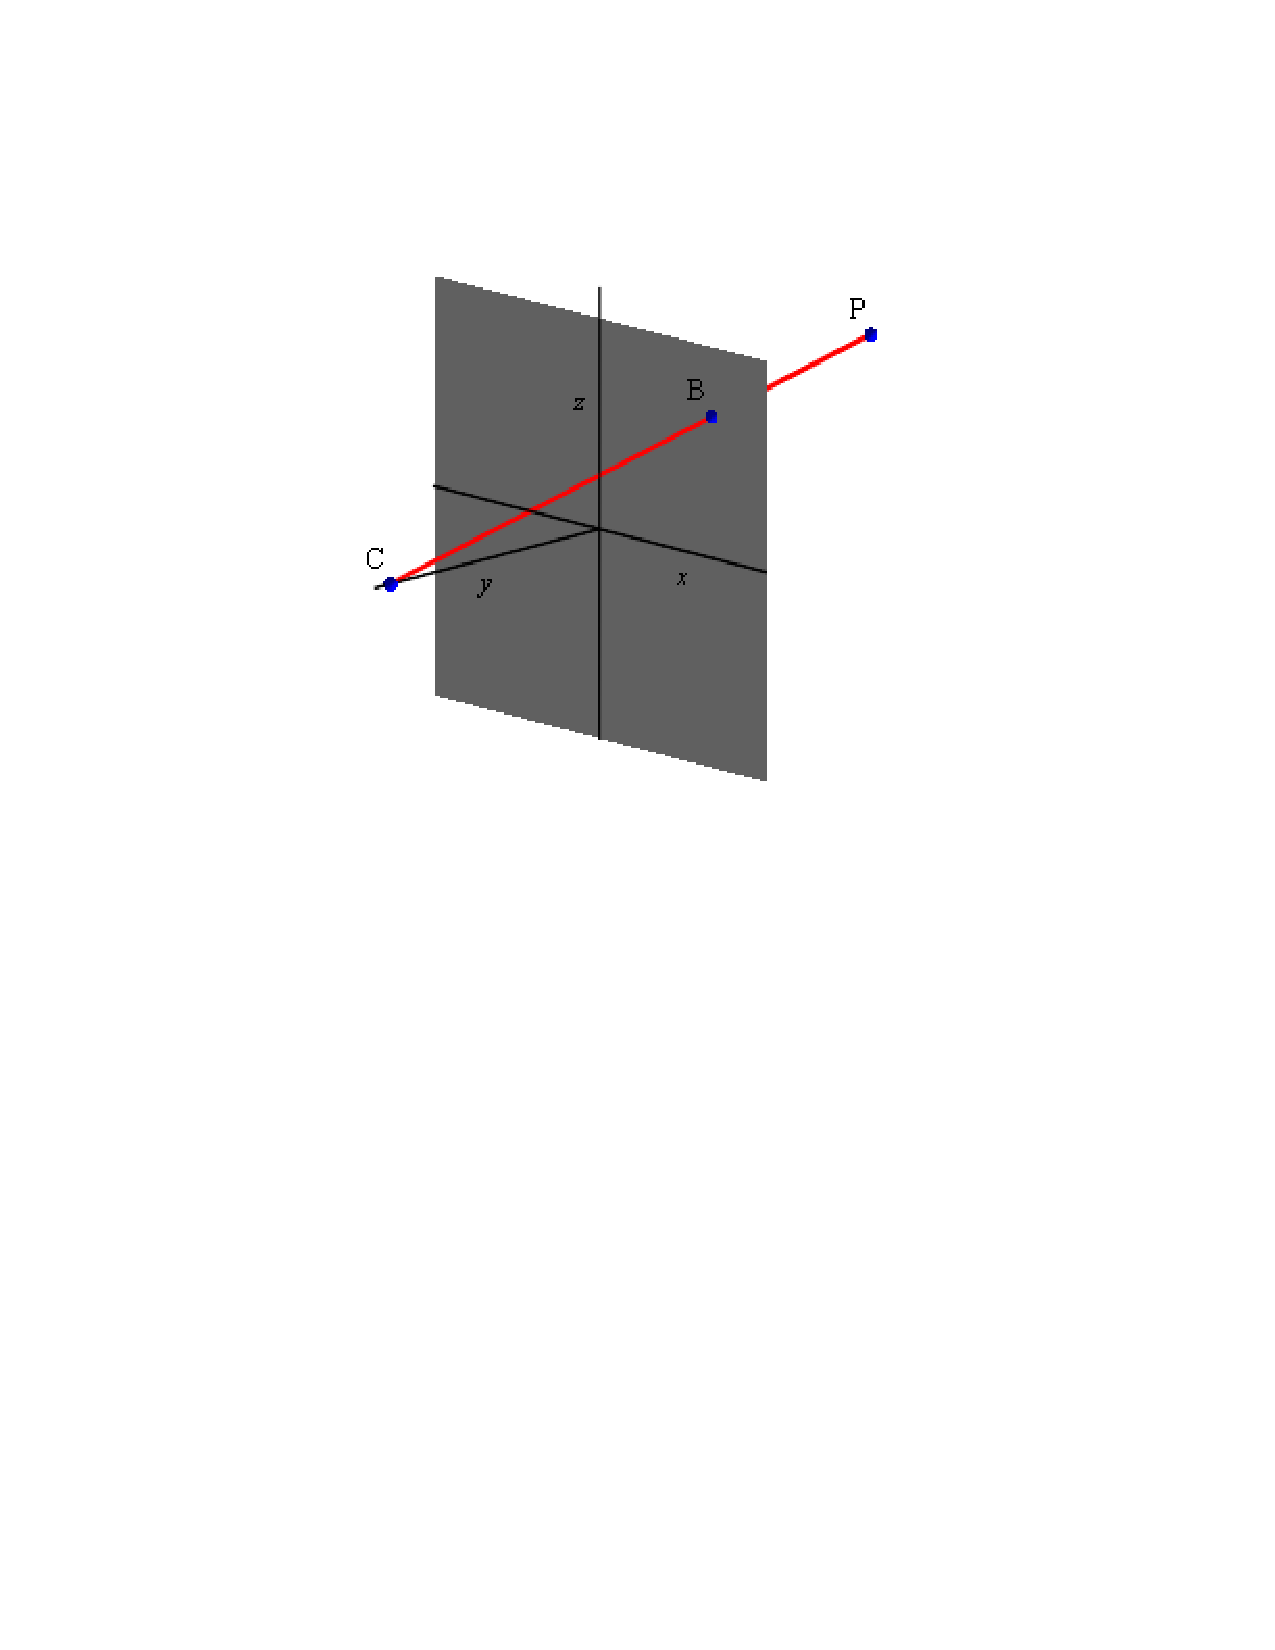
\includegraphics[width=5cm]{perspektiv_projektion}
  \caption{Viser princippet bag perspektiv projektion af et punkt på et billedplan.}
\end{figure}

Som vist på figur \ref{fig:perspektiv_projektion} kan et punkt $P\in \mathbb{R}^3$ projekteres ned på billedplanen $\alpha$ ved at finde skæringspunktet $B$ mellem billedplanen $\alpha$ og en lysstråle $L$, som går fra punktet $P$ mod kameraets position $C$. Gør man nu dette for alle punkter på et objekt i rummet, og tegner skæringspunkterne på billedplanen, dannes et billede af objektet. Udfordringen er så at afgøre hvilken farve punkterne på billedplanen skal have, da dette til dels afhænger af objektets farve, men også hvilket udefrakommende lys der rammer objektet. 

For at løse denne udfordring, benytter vi i dette projekt raytracing, der som beskrevet under afsnit \ref{sec:computergrafik}, bygger på at simulere lysstrålers interaktion med forskellige objekter i rummet. Hvordan dette fungere er beskrevet i næste afsnit, hvor der opstilles en model for en backwards raytracing.

\paragraph{Raytracing}
I modsætning til en perspektiv projektion af et punkt på et plan, er raytracing, hvor man i stedet for punktet i rummet, tager udgangspunkt i de lysstråler der danner billedet. Ved backwards raytracing følger man lysstrålerne baglæns og ser på, hvor stor en lysintensitet, den pågældende lysstråle har efter den har interageret med objekterne i rummet. Ud fra dette farves det tilhørende punkt på billedet, og på den måde kan man rendere et helt billede. På figur \ref{fig:raytracing_skitse} er det vist hvordan man kan konstruere en lysstråle ud fra et bestemt punkt på billedplanen, hvor lysstrålen er beskrevet ved en retningsvektor og et startpunkt.

\begin{figure}[H]
  \label{fig:raytracing_skitse}
  \centering
  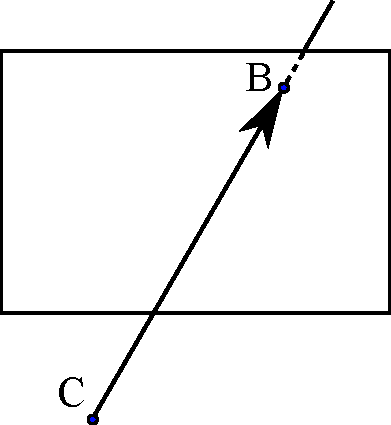
\includegraphics[width=5cm]{drawing}
  \caption{Viser hvordan en der kan opstilles retningsvektor mellem kameraets position $C$ og punktet $P$ på billedplanen, som sammen med startpunktet $C$ beskriver lysstrålen i omvendt retning.}
\end{figure}

Der findes flere forskellige modeller for hvordan lysintensiteten for en lysstråle beregnes. En simpel model, er Phong-modellen, som opdeler lys i forskellige kategorier: ambient, diffuse og specular.









